\documentclass[conference]{IEEEtran}
\usepackage{cite}
\usepackage{amsmath,amssymb,amsfonts}
\usepackage{algorithmic}
\usepackage{algorithm}
\usepackage{graphicx}
\usepackage{textcomp}
\usepackage{xcolor}
\usepackage{booktabs}
\usepackage{multirow}
\usepackage{hyperref}
\usepackage{subcaption}

% float placement tuning: pack figures at column tops/bottoms, never leave
% large white gaps, and avoid near-empty float-only pages.
\renewcommand{\topfraction}{0.95}
\renewcommand{\bottomfraction}{0.7}
\renewcommand{\textfraction}{0.07}
\renewcommand{\floatpagefraction}{0.8}
\setcounter{topnumber}{2}
\setcounter{bottomnumber}{1}
\setcounter{totalnumber}{3}

\definecolor{pendingcolor}{RGB}{200, 100, 50}
\newcommand{\pending}[1]{\textcolor{pendingcolor}{\textit{[#1]}}}

\begin{document}

\title{FAITH-SAE: Are Sparse-Autoencoder Concept\\ Directions in Vision Models Causally\\ Faithful Under Distribution Shift?}

\author{
\IEEEauthorblockN{Rajia Rani}
\IEEEauthorblockA{}
}

\maketitle

\begin{abstract}
\pending{DRAFT SCAFFOLD. This is a preview of how the final paper will look. The figures use illustrative placeholder numbers; the data figures and result tables are replaced with measured numbers once the experiments complete. The methodology schematic, background, and method are essentially final.}
Sparse autoencoders (SAEs) decompose a frozen vision model's activations into thousands of human-nameable concept directions, and one can \emph{steer} those concepts by editing the activations. But a steering edit and a faithfulness measure are each incomplete alone: a steering method with no metric is unfalsifiable, since a plausible-looking artifact is indistinguishable from a real causal effect; and a metric applied to a naive edit only scores off-manifold artifacts. This paper combines the two. The method is \emph{on-manifold steering}: rather than adding a raw activation-addition $\Delta$, we project the edit onto the top-$r$ principal directions of real-image activations ($P_M\,\Delta$), keeping the steered activation in the region the backbone was actually trained on. The measuring stick is the \emph{Causal Faithfulness Score} (CFS), a single number in $[0,1]$ that is the harmonic mean of monotonicity (knob up $\rightarrow$ readout up, smoothly), specificity (only the target concept moves), and sufficiency (effect size matches the concept's claimed meaning), so a near-zero in any axis drags the whole score down. We run, on a frozen CLIP ViT-B/16, the first faithfulness benchmark for vision SAE features, comparing on-manifold steering against naive off-manifold, random-direction, raw-clamp, and supervised TCAV-style steering at matched strength, and the first \emph{OOD-faithfulness sweep} across clean ImageNet $\rightarrow$ ImageNet-R $\rightarrow$ ImageNet-Sketch $\rightarrow$ ImageNet-C $\rightarrow$ ObjectNet, locating the collapse knee. \pending{We expect on-manifold steering to be substantially more faithful than naive steering at matched strength and to degrade more gracefully as inputs shift out of distribution; final numbers to be reported.}
\end{abstract}

\begin{IEEEkeywords}
sparse autoencoders, mechanistic interpretability, causal faithfulness, activation steering, distribution shift, vision transformers, CLIP, concept directions.
\end{IEEEkeywords}

\section{Introduction}

\begin{figure*}[t]
\centering
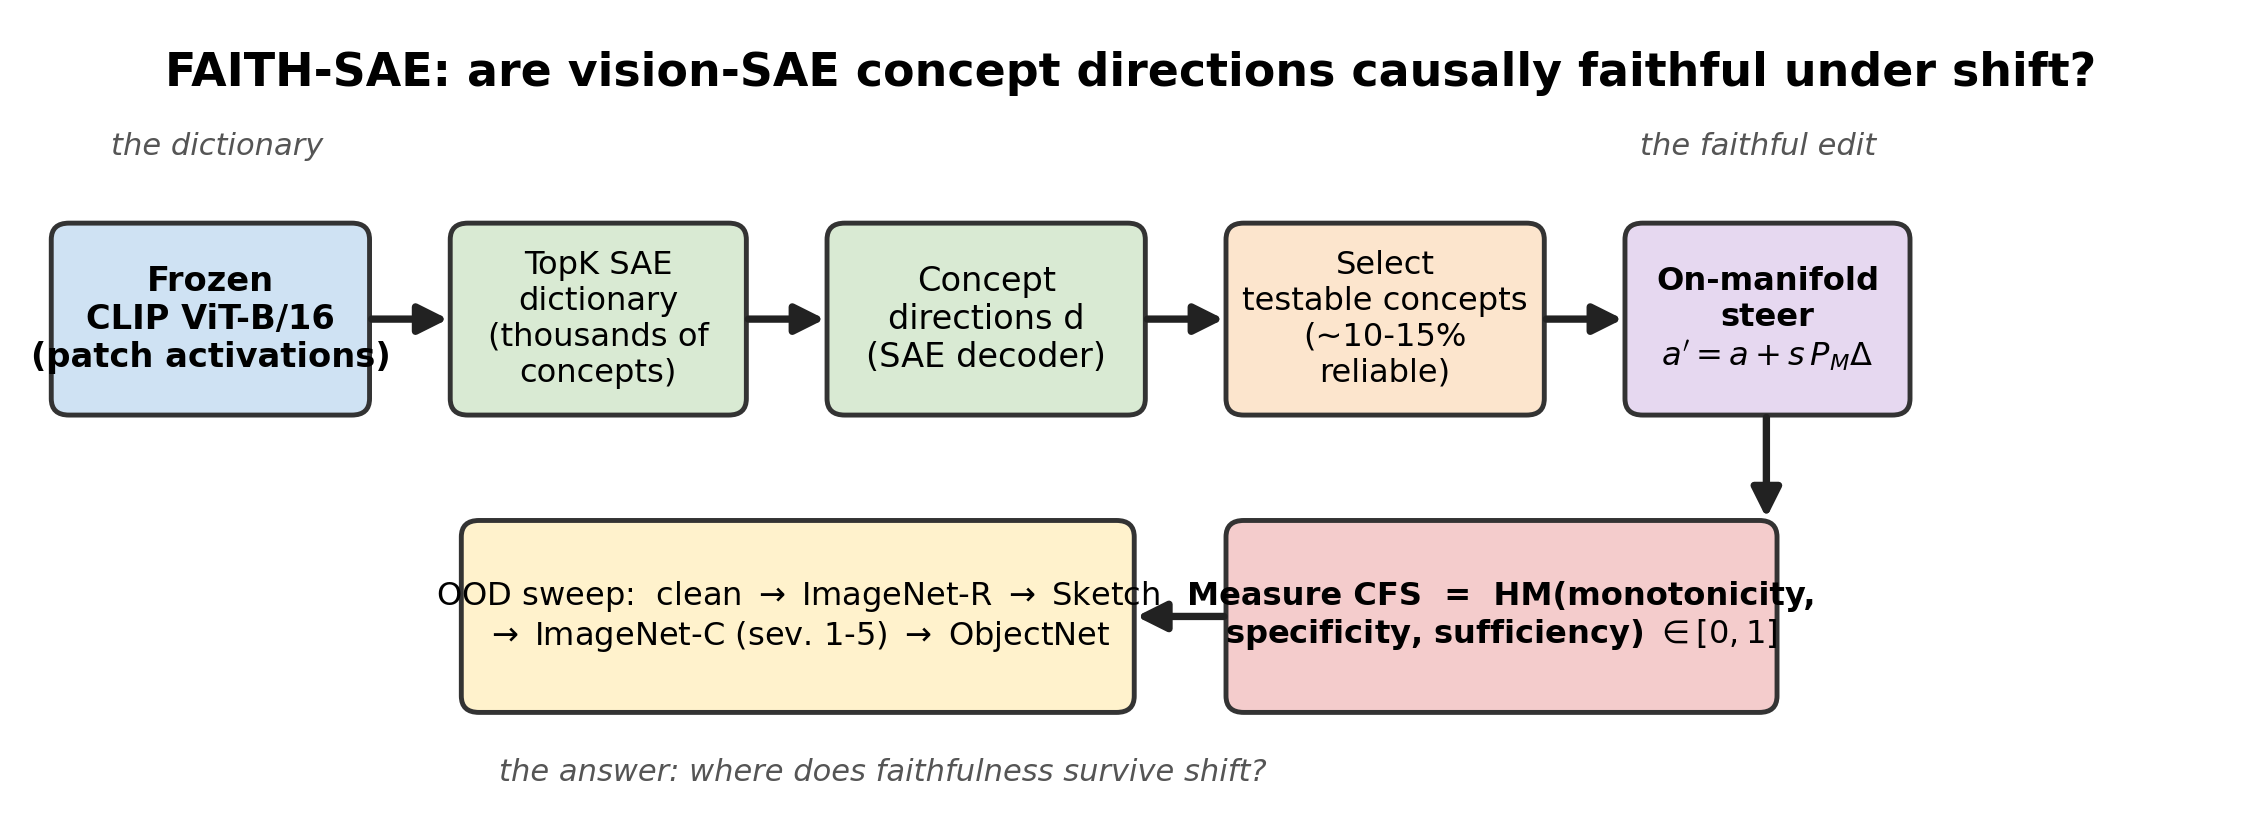
\includegraphics[width=0.98\textwidth]{figures/fig_overview.png}
\caption{Study overview. A frozen CLIP ViT-B/16 produces patch-token activations; a TopK sparse autoencoder decomposes them into thousands of concept directions. We select the well-defined concepts, steer each one \emph{on-manifold} by projecting the edit onto the top-$r$ real-image subspace, score it with the Causal Faithfulness Score (monotonicity $\times$ specificity $\times$ sufficiency), and then re-measure that score as inputs walk down an out-of-distribution ladder (clean ImageNet $\rightarrow$ R $\rightarrow$ Sketch $\rightarrow$ C $\rightarrow$ ObjectNet).}
\label{fig:overview}
\end{figure*}

Sparse autoencoders find interpretable features. Trained as an overcomplete, sparsely-activating dictionary over a frozen model's internal activations, an SAE recovers thousands of directions that often correspond to human-nameable concepts \cite{cunningham2023sae,bricken2023monosemanticity,templeton2024scaling}, and the same construction transfers to vision backbones, where features pick out textures, parts, and objects. Once a concept direction is in hand, the natural next move is \emph{steering}: push that direction up or down inside the network and watch the output change. This is the bridge from \emph{description} to \emph{intervention}, and there are two complementary things one must get right to cross it.

The first is the edit itself. The standard recipe is activation addition \cite{turner2023actadd,zou2023repe}: add a scaled concept direction to the residual stream, $a \leftarrow a + s\,d$. It is simple and it moves the output, but it is also \emph{off-manifold}, since nothing forces the steered activation to resemble anything the frozen backbone ever saw on a real image. The model can respond to an out-of-distribution activation in ways that have nothing to do with the named concept, so the visible effect may be a plausible artifact rather than a real causal lever (Fig.~\ref{fig:overview}). The second thing is the measurement. Even a perfect edit is scientifically empty without a way to ask whether the change is \emph{causally faithful} to the concept's claimed meaning. These two failures are linked: a steering method with no metric is unfalsifiable, while a metric applied to a naive edit just measures the artifact.

The fix that interpretability keeps rediscovering, in different guises, is \emph{stay close to the data distribution and check the effect three ways}. On-manifold thinking appears in representation engineering and in critiques of off-manifold patching \cite{zou2023repe,makelov2024principled}; the three-way check, that a real causal handle must respond \emph{monotonically}, act \emph{specifically}, and be \emph{sufficient}, appears piecemeal across causal-scrubbing \cite{chan2022scrubbing} and feature-attribution removal tests \cite{hooker2018roar}. No one has combined them for vision SAE features, and, crucially, no one has asked the question that matters most for trust: \textbf{does that faithfulness survive when the input image shifts out of distribution?} A concept lever that is faithful on clean ImageNet but collapses on a sketch or a corrupted photo is a lever you cannot trust in deployment.

The central question of this paper, stated plainly, is: \textbf{is steering a vision SAE concept on-manifold causally faithful where naive off-manifold steering is not, and how far does that faithfulness survive as the input distribution shifts?} We answer it with two mechanisms that cure each other's blind spot. On-manifold steering gives the metric something \emph{real} to measure; the Causal Faithfulness Score (CFS) proves the on-manifold edit is faithful and tracks exactly where it breaks under shift. The CFS-versus-shift curve is the paper's answer.

Our contributions are as follows.
\begin{enumerate}
\item A \textbf{Causal Faithfulness Score} for vision SAE features, the harmonic mean of monotonicity, specificity, and sufficiency (Sec.~\ref{sec:method}), \emph{paired with} an \textbf{on-manifold projected-steering} method $a' = a + s\,(P_M\,\Delta)$ that keeps edits realistic, decodable, and non-destructive, a measuring stick and a faithful editing method that did not exist together.
\item A \textbf{controlled on-manifold-vs-naive study}: at matched steering strength, on-manifold steering against naive off-manifold, random-direction, raw-clamp, and supervised TCAV-style steering, with bootstrap confidence intervals over concepts and the per-concept reliability distribution (the field's ``only $\sim$10--15\% steer cleanly'' claim).
\item The \textbf{first OOD-faithfulness benchmark} for vision SAE concepts: CFS measured across clean ImageNet $\rightarrow$ ImageNet-R $\rightarrow$ ImageNet-Sketch $\rightarrow$ ImageNet-C (a 1--5 severity dial) $\rightarrow$ ObjectNet, with the degradation slope and collapse knee, yielding an actionable answer either way.
\end{enumerate}

\section{Background and Related Work}

\subsection{Sparse autoencoders and monosemanticity}
SAEs learn an overcomplete dictionary whose codes are sparse, recovering directions that are far more monosemantic than raw neurons \cite{cunningham2023sae,bricken2023monosemanticity}. Scaling the dictionary and the sparsity mechanism, TopK and JumpReLU/Gated variants, improves the reconstruction--sparsity frontier and the fraction of clean features \cite{gao2024topk,rajamanoharan2024jumprelu,templeton2024scaling}. This line tells us SAEs \emph{find} concepts; it says little about whether \emph{intervening} on a found concept is causally faithful, and almost nothing in the vision setting.

\subsection{Activation steering and representation engineering}
Activation addition \cite{turner2023actadd} and representation engineering \cite{zou2023repe} edit a model by adding a concept direction to its activations. These methods are effective but admittedly fragile: the edited activation can leave the data manifold, and the resulting output change need not reflect the named concept. Our on-manifold projection is a direct response, constraining the edit to the subspace real images actually occupy.

\subsection{Supervised concept directions}
TCAV \cite{kim2017tcav} derives a concept activation vector from labelled examples via a linear probe, a label-expensive but strong direction. We use a TCAV-style supervised direction as the \emph{quality reference}: the gold an unsupervised SAE direction should approach. Sparse feature circuits \cite{marks2024circuits} and principled SAE evaluation \cite{makelov2024principled} similarly push toward causal, not merely correlational, accounts of features.

\subsection{Faithfulness and causal evaluation}
A description is faithful if intervening on it changes behaviour as the description predicts. Causal scrubbing \cite{chan2022scrubbing} formalises this for circuits; removal tests such as ROAR \cite{hooker2018roar} stress that an attribution must be checked by ablation, not assumed. Our CFS imports this spirit into a single $[0,1]$ score with conjunctive (harmonic-mean) semantics over three axes, so an edit is faithful only if it is monotone \emph{and} specific \emph{and} sufficient.

\subsection{Robustness and distribution shift}
The robustness literature provides exactly the stress ladder we need: ImageNet-R \cite{hendrycks2021many} (renditions/abstractions), ImageNet-Sketch \cite{wang2019sketch} (texture removed), ImageNet-C \cite{hendrycks2019benchmarking} (a graded corruption-severity dial), and ObjectNet \cite{barbu2019objectnet} (real-world pose/background/viewpoint). Texture-vs-shape bias \cite{geirhos2019texture} explains why sketch and rendition are hard. No prior work measures whether \emph{SAE-concept faithfulness} survives this ladder.

\subsection{Our position}
We combine the two mechanisms that are usually studied apart: an on-manifold steering method that keeps the edit realistic, and a faithfulness metric that makes ``faithful'' falsifiable, then we stress the pair across a distribution-shift ladder under one frozen backbone. The novel object is the interface: whether on-manifold steering is faithful where naive steering is not, and where that faithfulness collapses as inputs go out of distribution.

\section{Methodology}
\label{sec:method}

\begin{figure*}[t]
\centering
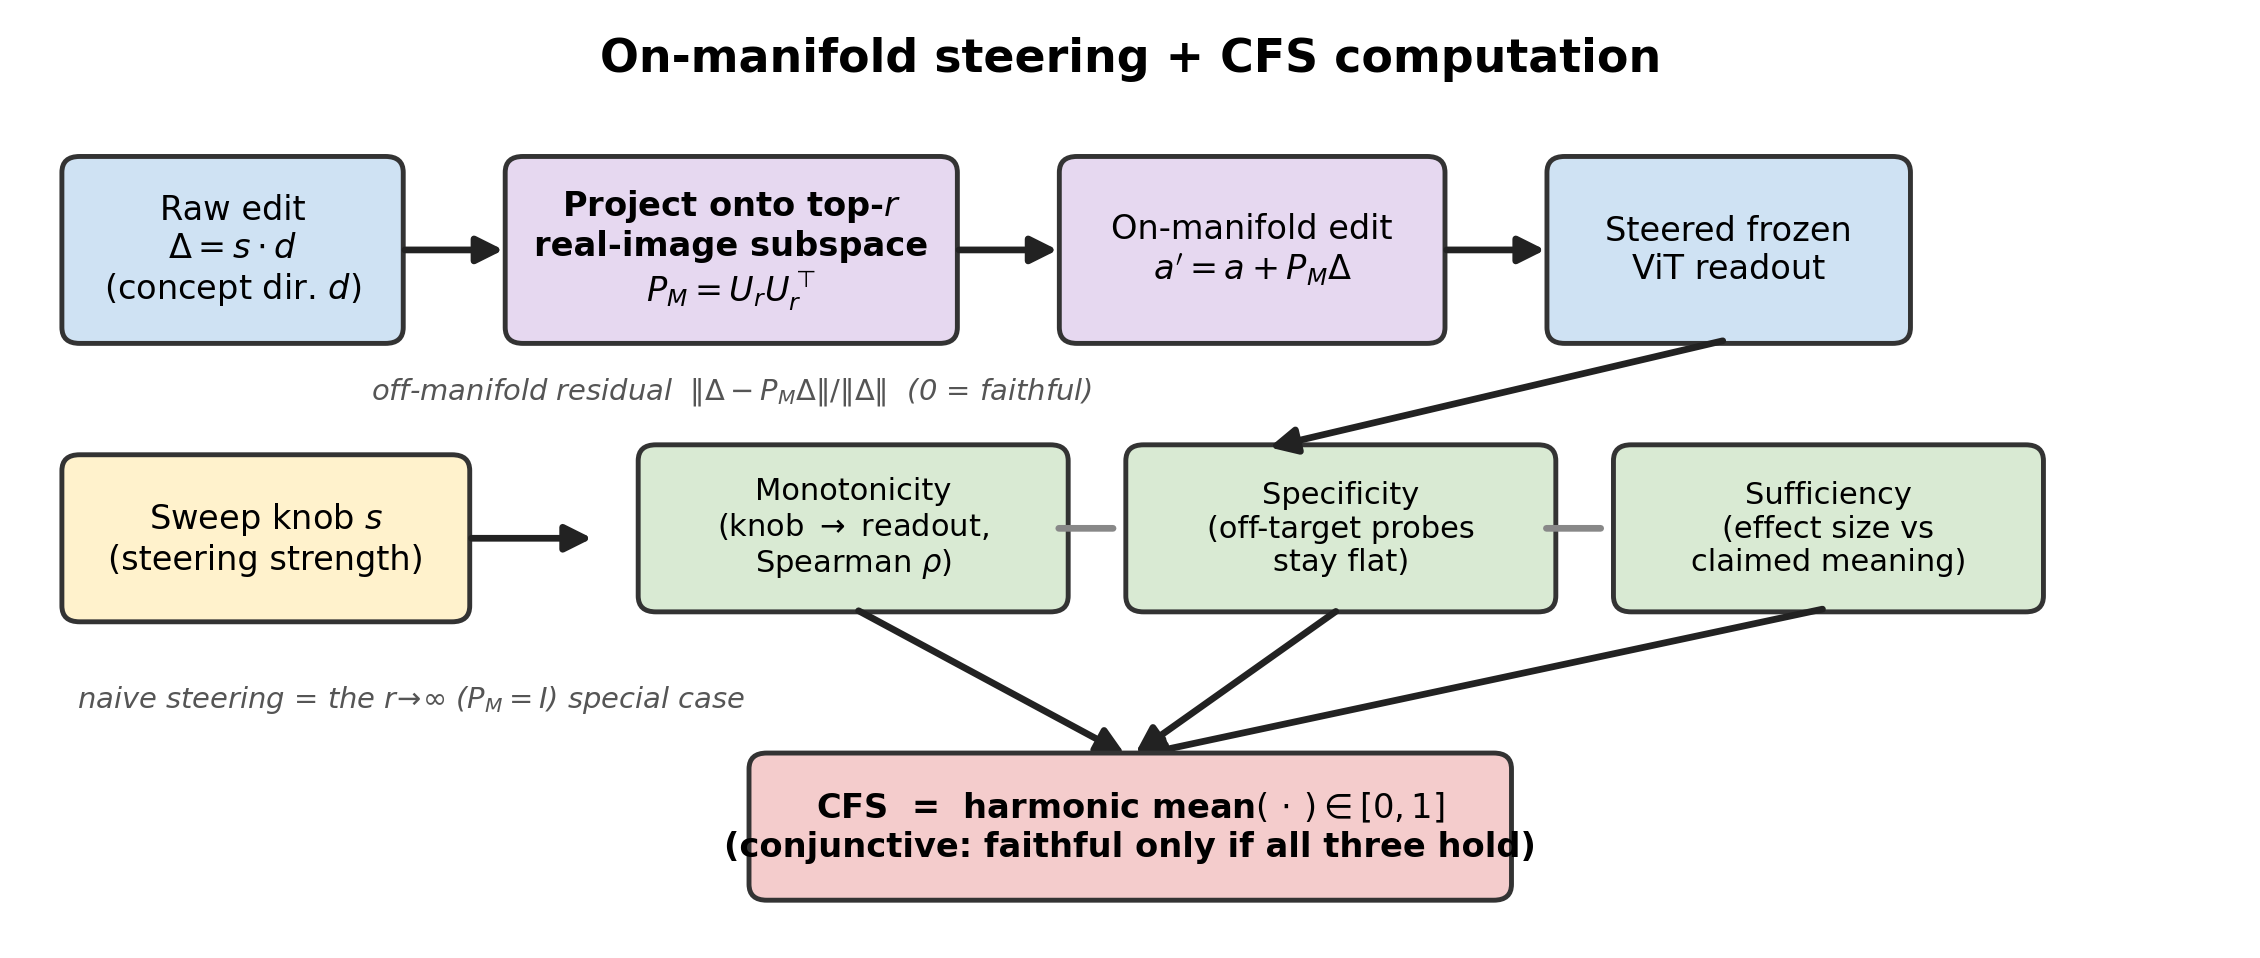
\includegraphics[width=0.96\textwidth]{figures/fig_method.png}
\caption{The on-manifold steering and CFS computation block. A raw activation-addition edit $\Delta = s\,d$ for an SAE concept direction $d$ is projected, $P_M\,\Delta$, onto the top-$r$ principal directions $U_r$ of real-image activations, so the steered activation $a' = a + s\,(P_M\,\Delta)$ stays on the manifold the backbone was trained on. Sweeping the knob $s$ produces a concept readout (monotonicity) and off-target probe drift (specificity); the standardized full-knob effect gives sufficiency. The three combine by harmonic mean into CFS $\in [0,1]$. Naive steering is the $r\!\rightarrow\!\infty$ ($P_M = I$) special case.}
\label{fig:method}
\end{figure*}

\subsection{Setup and the on-manifold edit}
We freeze a CLIP ViT-B/16 backbone and train a TopK sparse autoencoder on its patch-token activations at a chosen layer, yielding an overcomplete dictionary of concept directions $\{d_j\}$. To steer concept $j$, the naive recipe adds a scaled direction, $a \leftarrow a + s\,d_j$, where $s$ is the steering strength (the knob). The defect is that $a + s\,d_j$ may leave the region of activation space the frozen model ever sees on real images. We therefore estimate, from a held-out bank of real-image activations, the top-$r$ principal subspace with orthonormal basis $U_r$, define the projector $P_M = U_r U_r^{\top}$, and take the \emph{on-manifold} edit
\begin{equation}
a' \;=\; a + s\,(P_M\,\Delta), \qquad \Delta = d_j,\;\; P_M = U_r U_r^{\top},
\label{eq:onmanifold}
\end{equation}
which restricts the edit to the directions real images actually populate. Naive steering is the special case $r\!\rightarrow\!\infty$, $P_M = I$. The diagnostic that distinguishes the two is the off-manifold residual $\lVert \Delta - P_M\Delta\rVert / \lVert\Delta\rVert$, the fraction of the edit that lies outside the real-image subspace (0 = fully on-manifold).

\subsection{The Causal Faithfulness Score}
A steering edit is causally faithful if it is real, specific, and sufficient. We make this a single number. For a concept $j$ define, over a swept knob grid:
\emph{Monotonicity} $m$, the Spearman correlation between the knob $s$ and a held-out concept readout (a smooth, ordered response);
\emph{Specificity} $p$, one minus the normalized drift of \emph{off-target} linear probes (only the target concept should move);
and \emph{Sufficiency} $u$, a standardized (Cohen's-$d$-style) effect size of the readout at full knob against the concept's claimed magnitude. Each is clipped to $[0,1]$ and combined by a weighted harmonic mean,
\begin{equation}
\mathrm{CFS} \;=\; \mathrm{HM}(m, p, u) \;=\; \frac{\sum_i w_i}{\dfrac{w_m}{m} + \dfrac{w_p}{p} + \dfrac{w_u}{u}} \;\in\; [0,1],
\label{eq:cfs}
\end{equation}
whose conjunctive (AND) semantics mean that a near-zero in any one axis, e.g. an unspecific edit, drags the whole score toward zero: faithfulness requires all three at once. CFS is backbone- and library-independent, a per-concept, per-shift-level quantity, the paper's contributed measuring stick.

\subsection{The per-concept faithfulness path}
Algorithm~\ref{alg:cfs} states how CFS is computed for one concept under one steering variant on one shift level. The same path, run across the OOD ladder, produces the headline curve $\mathrm{CFS}(\text{shift})$ and its degradation slope $\Delta\mathrm{CFS}/\Delta\text{shift}$.

\begin{algorithm}[t]
\caption{CFS of a steering variant for concept $j$}
\label{alg:cfs}
\begin{algorithmic}
\STATE \textbf{Input:} concept $d_j$, knob grid $\{s_i\}$, basis $U_r$, images $X$
\STATE form projector $P_M \leftarrow U_r U_r^{\top}$ (identity for naive)
\FOR{each strength $s_i$ in the grid}
  \STATE edit activations $a' \leftarrow a + s_i\,(P_M\,d_j)$ over $X$
  \STATE record concept readout and off-target probe values
\ENDFOR
\STATE $m \leftarrow$ Spearman(knob, readout) \COMMENT{monotonicity}
\STATE $p \leftarrow 1 - $ normalized off-target drift \COMMENT{specificity}
\STATE $u \leftarrow$ standardized full-knob effect size \COMMENT{sufficiency}
\STATE \textbf{return} $\mathrm{CFS} \leftarrow \mathrm{HM}(m, p, u)$
\end{algorithmic}
\end{algorithm}

\subsection{The core design knob}
The two knobs that set faithfulness are the steering strength $s$ and the projection rank $r$. Strength trades effect against artifact: too small and the readout barely moves (sufficiency fails), too large and it saturates or clips and entangles off-target probes (monotonicity and specificity break, the magnitude-saturation knee). Rank trades on-manifold fidelity against expressivity: low $r$ over-constrains and the effect dies, high $r$ lets the edit drift off-manifold toward the naive limit. The $r \times s$ grid is the core design surface; its CFS knee is the operating point we report.

\subsection{Cost model}
The contributed quantity is implementation-independent by construction. CFS is a function only of readouts and probe drifts under steering, so it does not depend on kernel, library, or hardware, only on the backbone, the SAE, and the chosen knobs. The per-concept compute is a single knob sweep of forward passes through the frozen backbone plus a one-time $r$-dimensional PCA of a real-image activation bank; the projector $P_M$ is reused across all concepts and shift levels. We report CFS (and its three components, plus the off-manifold residual) per concept and per shift level, alongside the degradation slope and bootstrap confidence intervals over concepts.

\section{Experimental Setup}

\subsection{Backbone, SAE, and metrics}
The backbone is a frozen CLIP ViT-B/16; a TopK SAE is trained on its patch-token activations at a fixed layer. We report the three faithfulness components, the composite CFS, the off-manifold residual, the per-concept reliable fraction, and the OOD degradation slope with bootstrap confidence intervals over concepts. The distribution-shift ladder is in Table~\ref{tab:data}.

\begin{table}[t]
\caption{Benchmarks: the distribution-shift ladder.}
\label{tab:data}
\centering
\setlength{\tabcolsep}{3pt}
\begin{tabular}{lll}
\toprule
Benchmark & Family & Stresses \\
\midrule
ImageNet-val & clean in-distribution & quality reference \\
ImageNet-R & rendition / abstraction & style/domain shift \\
ImageNet-Sketch & texture removed & readout w/o texture \\
ImageNet-C & corruption dial (1--5) & graded OOD curve \\
ObjectNet & real-world pose/bg & faithfulness floor \\
\bottomrule
\end{tabular}
\end{table}

\subsection{Steering variants and protocol}
All steering variants are compared at \emph{matched} steering strength. Supervised TCAV-style steering is the quality reference; naive off-manifold activation addition is the main competitor; random-direction steering is the null/sanity baseline; raw-clamp steering clamps the SAE feature to a fixed magnitude with no projection; on-manifold projected steering (ours) constrains the edit to the top-$r$ real-image subspace. Principal settings and the swept knobs are in Table~\ref{tab:hparams}.

\begin{table}[t]
\caption{Principal hyperparameters and swept knobs.}
\label{tab:hparams}
\centering
\begin{tabular}{ll}
\toprule
Setting & Value \\
\midrule
Backbone & CLIP ViT-B/16 (frozen) \\
SAE type & TopK (vs L1, ablation) \\
TopK $k$ & swept (ablation) \\
Projection rank $r$ & swept (core knob) \\
Steering strength $s$ & swept (matched across variants) \\
Concept-select threshold & swept (ablation) \\
Backbone layer / token & swept; patch vs CLS (ablation) \\
Baselines & TCAV, naive, random, clamp \\
\bottomrule
\end{tabular}
\end{table}

\section{Results}
\label{sec:results}

\pending{All numbers and the data figures in this section are illustrative placeholders that show the intended analysis; they are replaced with measured results from results/metrics\_all.csv once the experiments run. The methodology schematic (Fig.~\ref{fig:method}) is final.}

\begin{table}[t]
\caption{Main result table (to be completed). CFS and its components, plus the off-manifold residual, per steering method on clean ImageNet at matched strength.}
\label{tab:main}
\centering
\setlength{\tabcolsep}{3pt}
\begin{tabular}{lccccc}
\toprule
Method & CFS & Mono. & Spec. & Suff. & Off-man. \\
\midrule
Supervised (TCAV, ref.) & \pending{tbd} & \pending{tbd} & \pending{tbd} & \pending{tbd} & \pending{tbd} \\
On-manifold (ours) & \pending{tbd} & \pending{tbd} & \pending{tbd} & \pending{tbd} & \pending{tbd} \\
Raw clamp & \pending{tbd} & \pending{tbd} & \pending{tbd} & \pending{tbd} & \pending{tbd} \\
Naive off-manifold & \pending{tbd} & \pending{tbd} & \pending{tbd} & \pending{tbd} & \pending{tbd} \\
Random direction & \pending{tbd} & \pending{tbd} & \pending{tbd} & \pending{tbd} & \pending{tbd} \\
\bottomrule
\end{tabular}
\end{table}

\subsection{CFS across the OOD sweep}
Figure~\ref{fig:oodsweep} is the headline: CFS against shift severity, walking clean ImageNet $\rightarrow$ R $\rightarrow$ Sketch $\rightarrow$ C-1..5 $\rightarrow$ ObjectNet, for on-manifold versus naive steering, with the collapse knee marked and a bootstrap confidence band. \pending{We expect on-manifold steering to stay above the usability floor further along the ladder than naive, with a later collapse knee.}

\begin{figure}[t]
\centering

\includegraphics[width=\columnwidth]{figures/fig1_cfs_ood_sweep.png}
\caption{Headline: CFS versus shift severity (clean $\rightarrow$ R $\rightarrow$ Sketch $\rightarrow$ C-1..5 $\rightarrow$ ObjectNet) for on-manifold versus naive steering; collapse knee marked, bootstrap CI band. \pending{Illustrative.}}
\label{fig:oodsweep}
\end{figure}

\subsection{The faithfulness Pareto front}
Figure~\ref{fig:pareto} plots specificity against effect-size/monotonicity across all five steering methods. A faithful method must be high on both; random sits in the corner (effect with no specificity), naive trades specificity for effect, and on-manifold should sit on the frontier near the supervised reference. \pending{We expect on-manifold steering on the Pareto frontier and random-direction steering in the low-specificity corner.}

\begin{figure}[t]
\centering
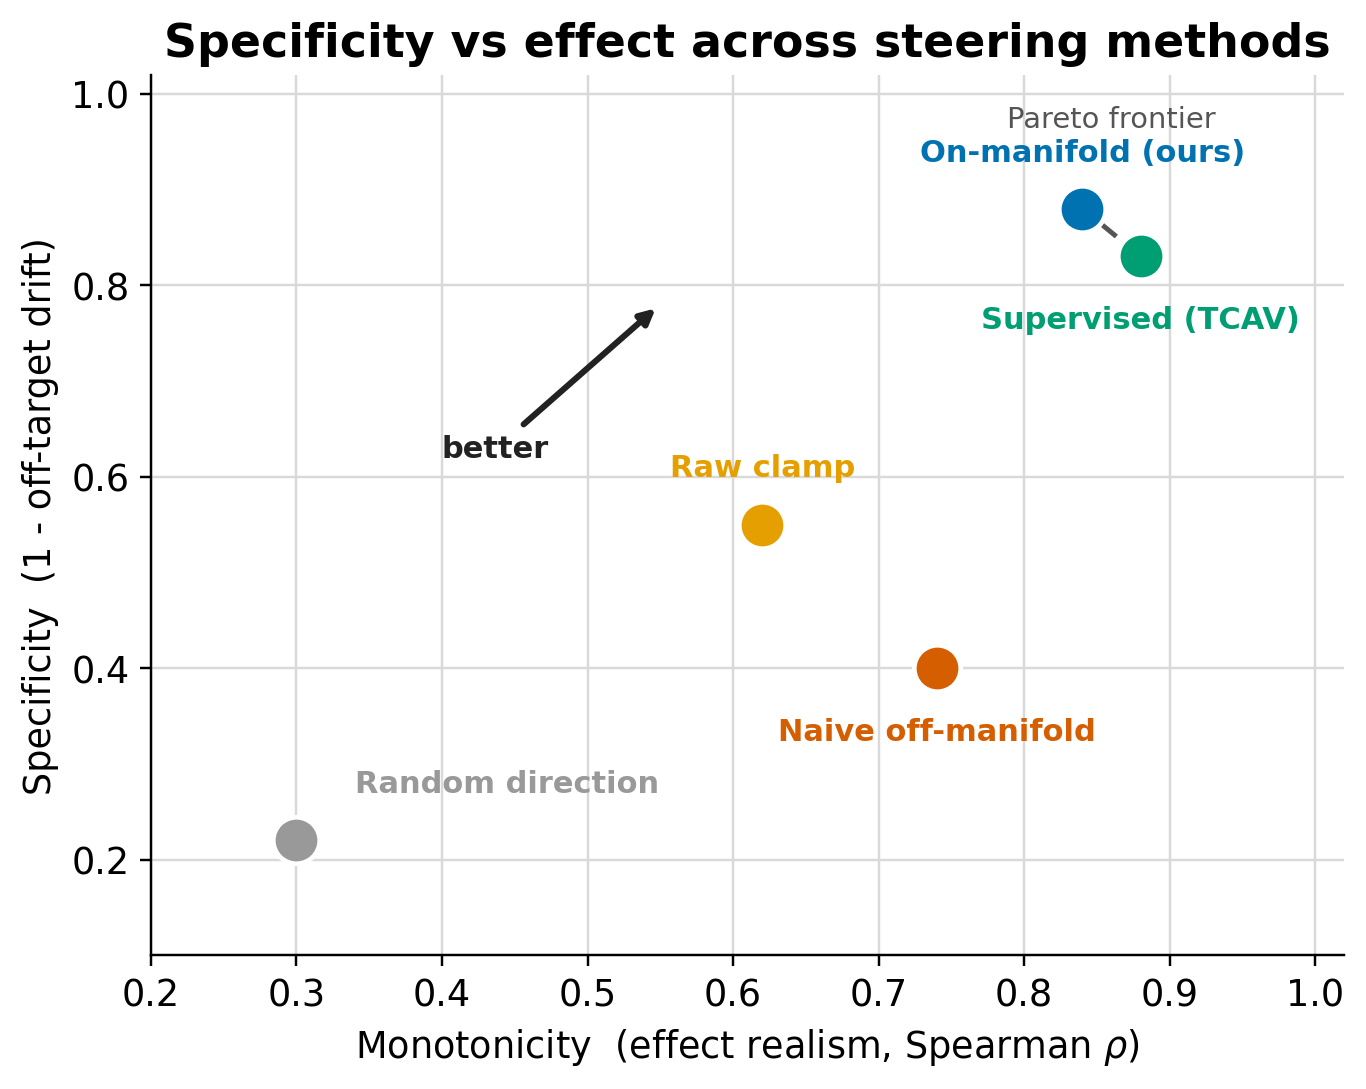
\includegraphics[width=\columnwidth]{figures/fig2_faithfulness_pareto.png}
\caption{Specificity versus effect-size/monotonicity across the five steering methods; up and to the right is faithful. \pending{Illustrative.}}
\label{fig:pareto}
\end{figure}

\subsection{The strength sweep and saturation knee}
Figure~\ref{fig:strength} sweeps the steering strength $s$ and marks the magnitude-saturation knee, where the readout flattens or clips and monotonicity breaks. The faithfulness optimum is a moderate strength, not the largest. \pending{We expect a single interior CFS optimum with a marked saturation knee beyond it.}

\begin{figure}[t]
\centering
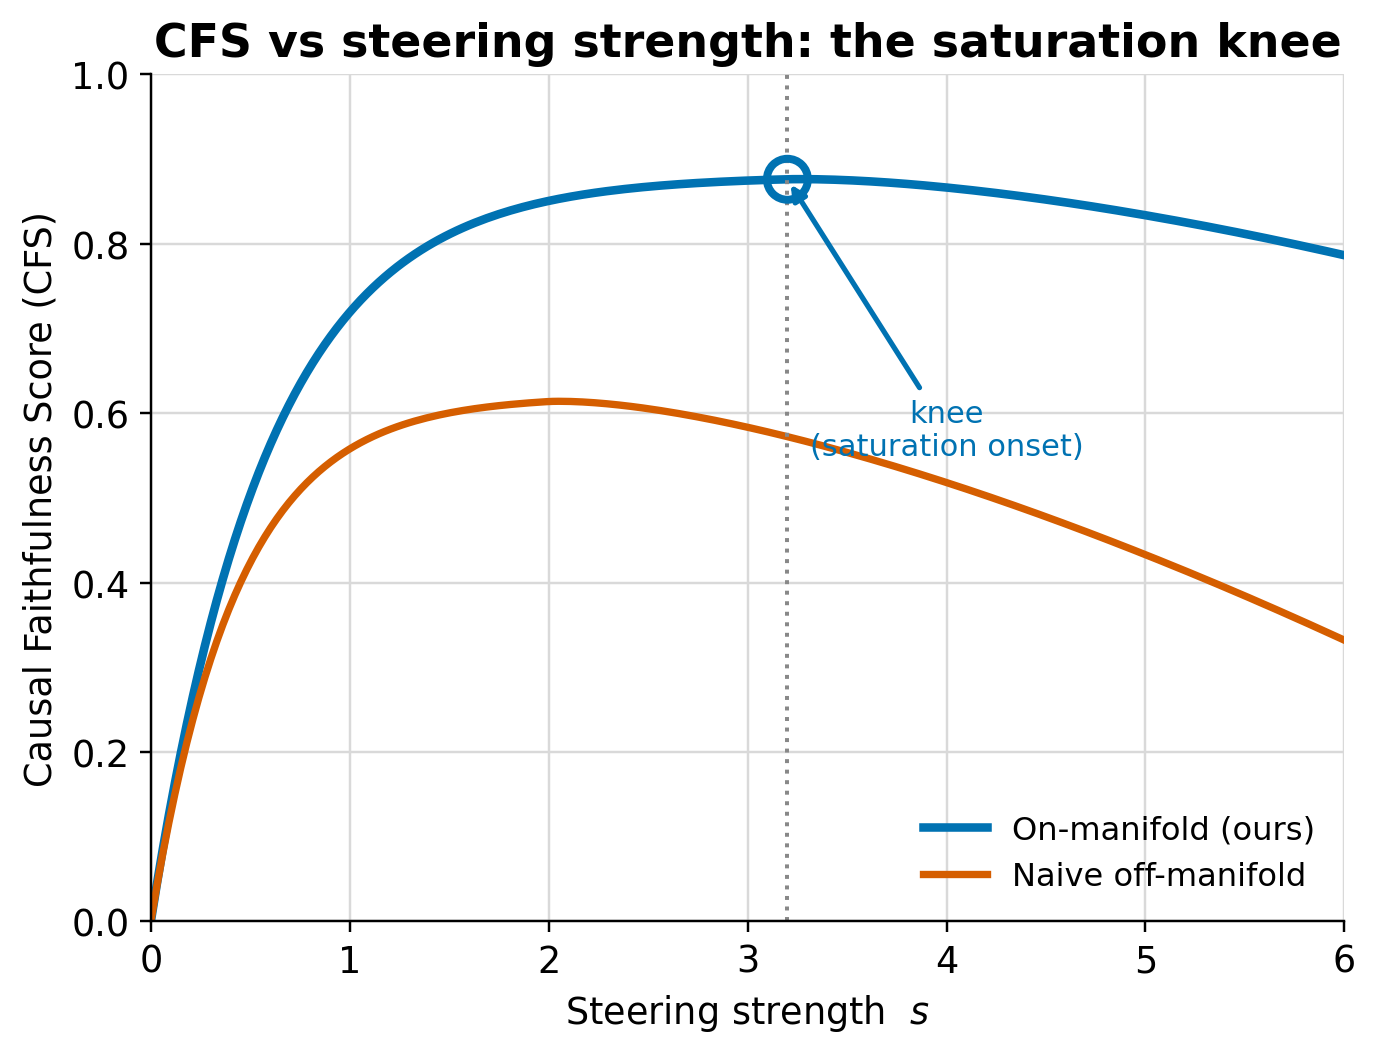
\includegraphics[width=\columnwidth]{figures/fig3_strength_sweep.png}
\caption{CFS versus steering strength $s$ with the magnitude-saturation knee marked. \pending{Illustrative.}}
\label{fig:strength}
\end{figure}

\subsection{Per-concept reliability}
Figure~\ref{fig:reliability} shows the distribution of per-concept CFS: a long mass of unreliable concepts and a small reliable tail, testing the field's ``only $\sim$10--15\% steer cleanly'' claim and the effect of the concept-selection threshold. \pending{We expect a heavy-tailed distribution with a small high-CFS reliable fraction.}

\begin{figure}[t]
\centering
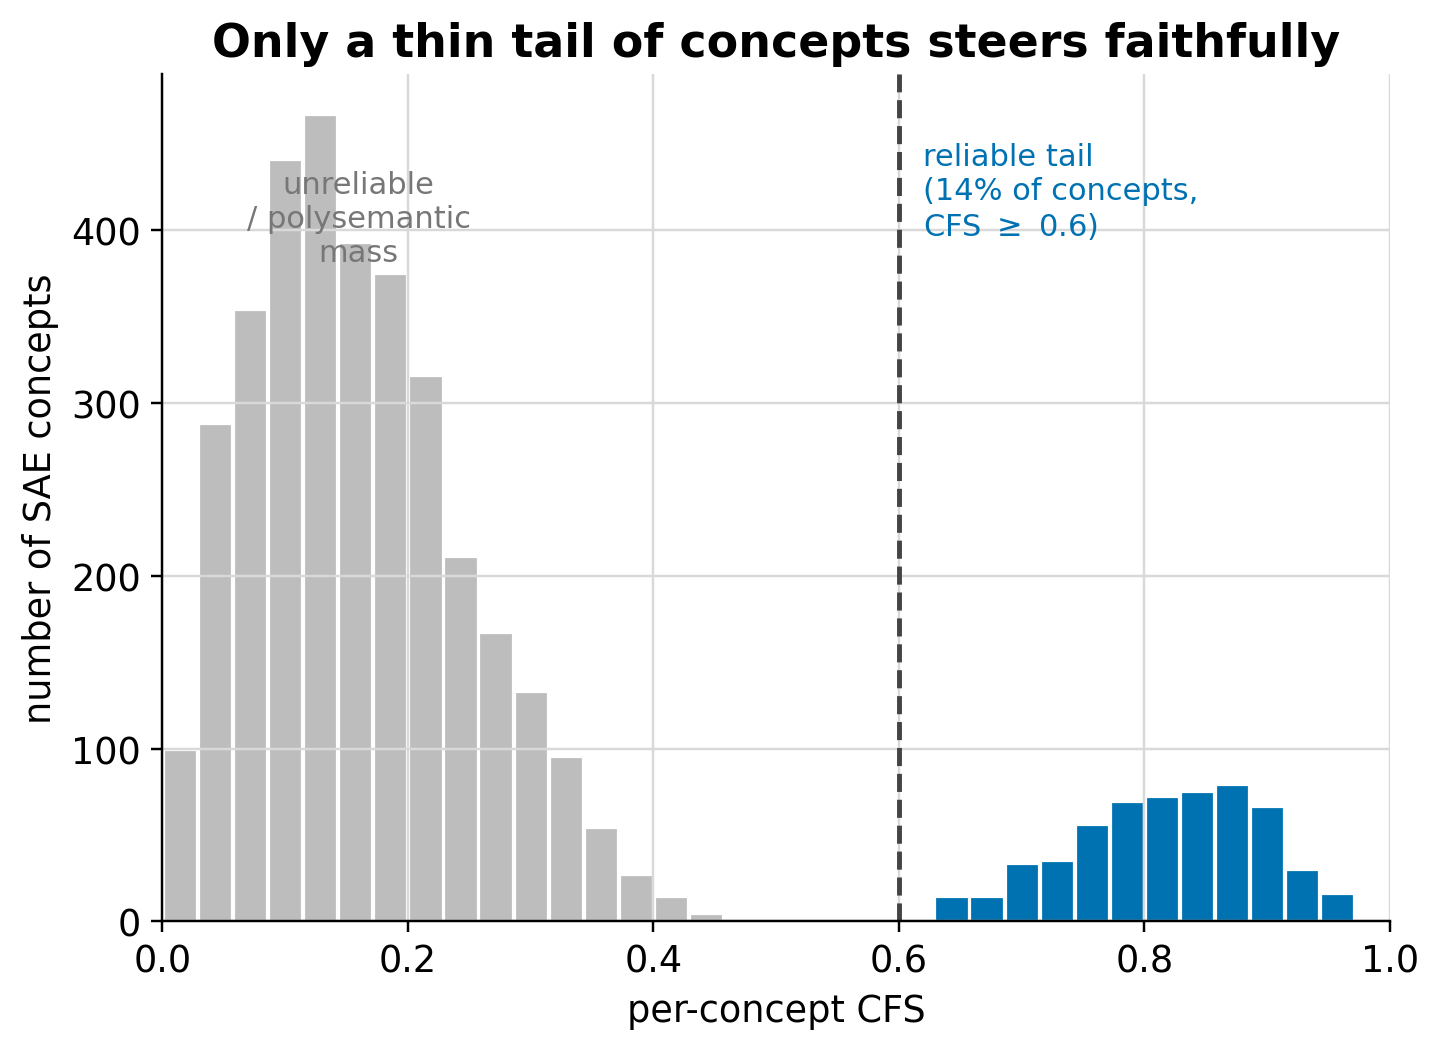
\includegraphics[width=\columnwidth]{figures/fig4_concept_reliability.png}
\caption{Distribution of per-concept CFS: the long unreliable mass and the small reliable tail. \pending{Illustrative.}}
\label{fig:reliability}
\end{figure}

\subsection{The shift $\times$ method heatmap}
Figure~\ref{fig:heatmap} is a 2-D grid, shift type (rows) by steering method (columns), with CFS as the cell value and the best cell (on-manifold, clean) boxed. It summarizes where faithfulness lives and dies across the whole design. \pending{We expect the on-manifold column to dominate at every shift level and the high-severity rows to be the darkest.}

\begin{figure}[t]
\centering
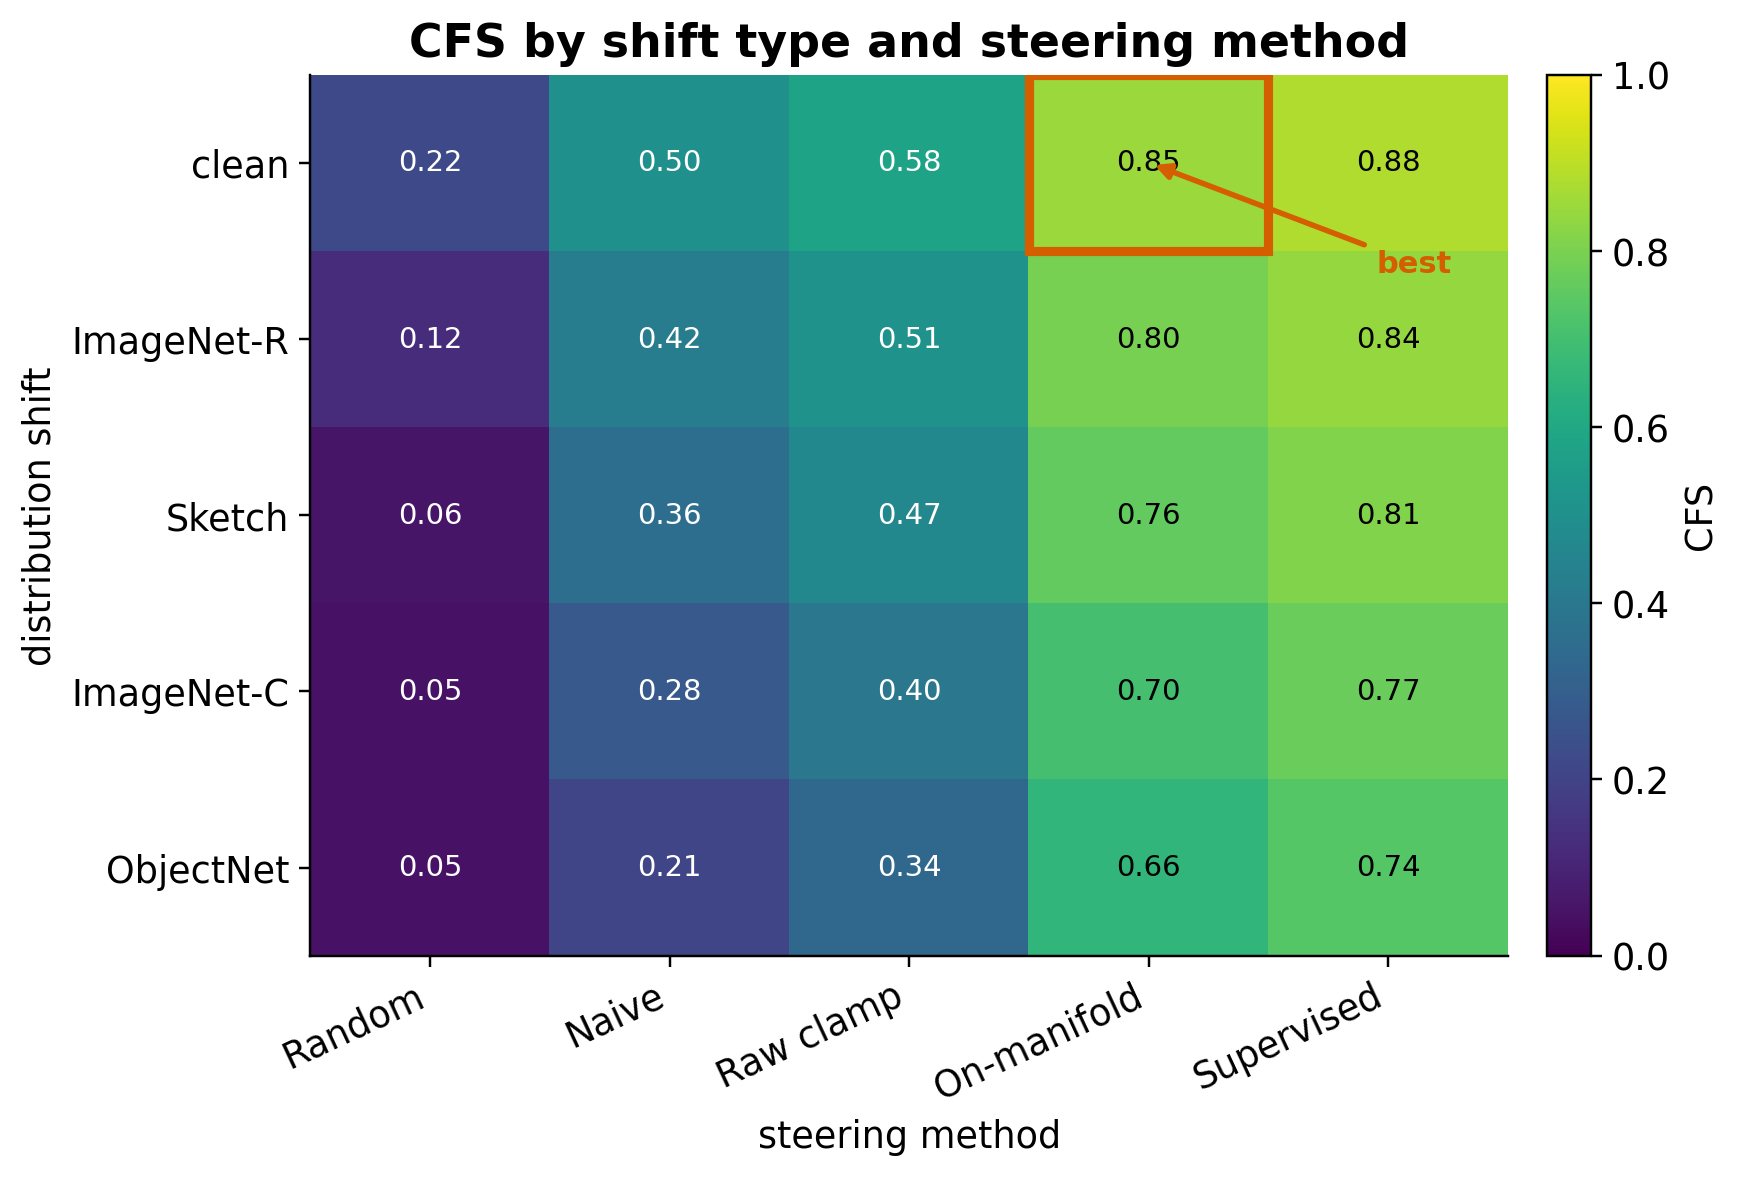
\includegraphics[width=\columnwidth]{figures/fig5_ood_heatmap.png}
\caption{CFS heatmap over shift type (rows) by steering method (columns); best cell boxed. \pending{Illustrative.}}
\label{fig:heatmap}
\end{figure}

\subsection{Monotonicity, smooth versus jagged}
Figure~\ref{fig:monotonicity} shows the concept readout against the knob for an example concept: smooth and monotone for on-manifold steering, jagged and non-monotone for naive. This is the visual signature of a real causal lever versus an artifact. \pending{We expect a smooth monotone on-manifold curve and a jagged non-monotone naive curve.}

\begin{figure}[t]
\centering
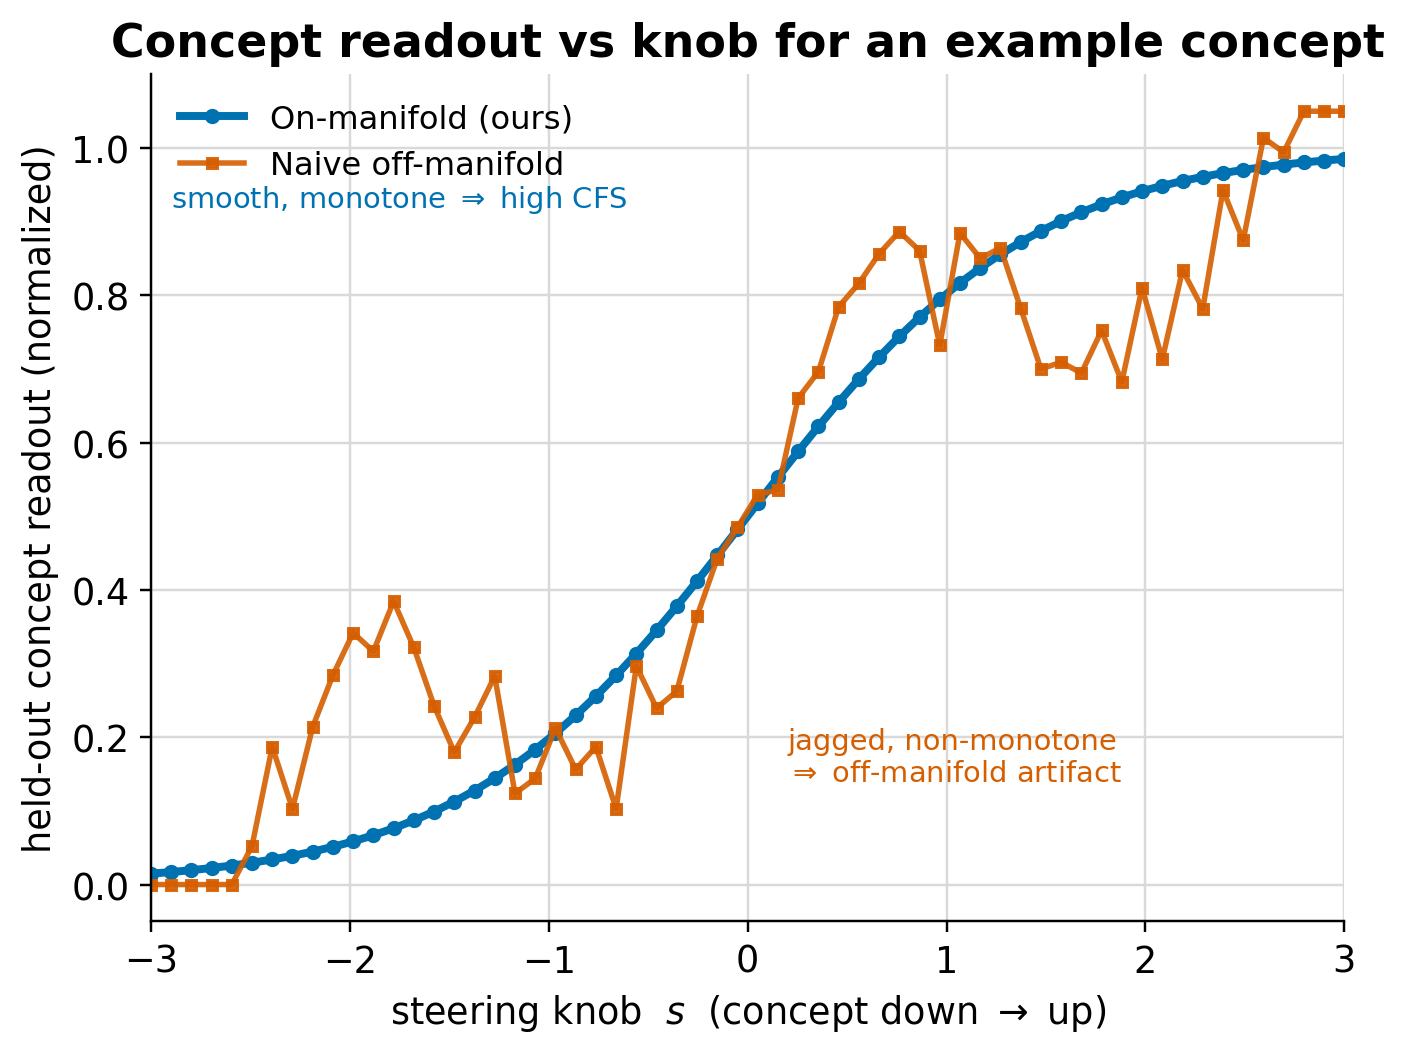
\includegraphics[width=\columnwidth]{figures/fig6_monotonicity_curve.png}
\caption{Concept readout versus knob for an example concept: on-manifold (smooth, monotone) versus naive (jagged). \pending{Illustrative.}}
\label{fig:monotonicity}
\end{figure}

\subsection{Mean CFS by method}
Figure~\ref{fig:bymethod} reports mean CFS by steering variant, supervised / on-manifold / clamp / naive / random, with bootstrap confidence intervals over concepts, the controlled summary of the matched-strength comparison. \pending{We expect on-manifold close behind supervised and clearly above clamp, naive, and random, with non-overlapping CIs.}

\begin{figure}[t]
\centering

\includegraphics[width=\columnwidth]{figures/fig7_by_method_bar.png}
\caption{Mean CFS by steering variant with bootstrap confidence intervals over concepts. \pending{Illustrative.}}
\label{fig:bymethod}
\end{figure}

\section{Discussion and Limitations}
This study is run at small scale on a single frozen backbone (CLIP ViT-B/16) and one SAE family, so its claims are about the faithfulness of on-manifold steering for that backbone under the stated training and selection choices, not a universal law. CFS is implementation-independent by construction, but it inherits the assumptions of its three components, the choice of held-out readout, off-target probe set, and claimed-magnitude reference for sufficiency, and a different probe set could move the score. The method has an intrinsic boundary: the manifold projector $P_M$ is estimated from \emph{in-distribution} real images, so under heavy shift the very subspace we project onto may no longer describe the test data, which is precisely the regime where we expect, and aim to measure, faithfulness collapse. The concept-selection threshold trades coverage against reliability, and the reliable-fraction claim depends on it. \pending{Add observed limitations after running: the measured reliable fraction, the shift level of the collapse knee, the sensitivity of CFS to the probe set, and SAE-maturity effects.}

\section{Conclusion}
We combined the two halves that are incomplete alone, a faithful editing method and a faithfulness metric, into one study of vision SAE concepts. On-manifold steering projects the edit onto the top-$r$ real-image subspace so the edit stays realistic; the Causal Faithfulness Score makes ``faithful'' a single conjunctive number over monotonicity, specificity, and sufficiency; and the OOD sweep measures, for the first time, whether that faithfulness survives as images shift from clean ImageNet down to renditions, sketches, corruptions, and real-world ObjectNet. \pending{State the final answer: whether on-manifold steering is faithful where naive is not, the reliable-concept fraction, and where on the OOD ladder faithfulness collapses, so trustworthy or a warning to the field.}

\section*{Acknowledgments}
The author thanks their mentors and collaborators for guidance and computational resources.

\begin{thebibliography}{99}
\bibitem{cunningham2023sae} H. Cunningham, A. Ewart, L. Riggs, R. Huben, and L. Sharkey, ``Sparse autoencoders find highly interpretable features in language models,'' \textit{Proc. ICLR}, 2024. arXiv:2309.08600.
\bibitem{bricken2023monosemanticity} T. Bricken et al., ``Towards monosemanticity: decomposing language models with dictionary learning,'' \textit{Transformer Circuits Thread}, Anthropic, 2023.
\bibitem{gao2024topk} L. Gao et al., ``Scaling and evaluating sparse autoencoders,'' \textit{Proc. ICLR}, 2025. arXiv:2406.04093.
\bibitem{templeton2024scaling} A. Templeton et al., ``Scaling monosemanticity: extracting interpretable features from Claude 3 Sonnet,'' \textit{Transformer Circuits Thread}, Anthropic, 2024.
\bibitem{turner2023actadd} A. M. Turner et al., ``Activation addition: steering language models without optimization,'' arXiv:2308.10248, 2023.
\bibitem{zou2023repe} A. Zou et al., ``Representation engineering: a top-down approach to AI transparency,'' arXiv:2310.01405, 2023.
\bibitem{kim2017tcav} B. Kim et al., ``Interpretability beyond feature attribution: quantitative testing with concept activation vectors (TCAV),'' \textit{Proc. ICML}, 2018. arXiv:1711.11279.
\bibitem{radford2021clip} A. Radford et al., ``Learning transferable visual models from natural language supervision (CLIP),'' \textit{Proc. ICML}, 2021. arXiv:2103.00020.
\bibitem{dosovitskiy2020vit} A. Dosovitskiy et al., ``An image is worth 16x16 words: transformers for image recognition at scale (ViT),'' \textit{Proc. ICLR}, 2021. arXiv:2010.11929.
\bibitem{hendrycks2021many} D. Hendrycks et al., ``The many faces of robustness: a critical analysis of out-of-distribution generalization (ImageNet-R),'' \textit{Proc. ICCV}, 2021. arXiv:2006.16241.
\bibitem{hendrycks2019benchmarking} D. Hendrycks and T. Dietterich, ``Benchmarking neural network robustness to common corruptions and perturbations (ImageNet-C),'' \textit{Proc. ICLR}, 2019. arXiv:1903.12261.
\bibitem{wang2019sketch} H. Wang, S. Ge, Z. Lipton, and E. P. Xing, ``Learning robust global representations by penalizing local predictive power (ImageNet-Sketch),'' \textit{Proc. NeurIPS}, 2019. arXiv:1905.13549.
\bibitem{barbu2019objectnet} A. Barbu et al., ``ObjectNet: a large-scale bias-controlled dataset for pushing the limits of object recognition models,'' \textit{Proc. NeurIPS}, 2019.
\bibitem{chan2022scrubbing} L. Chan et al., ``Causal scrubbing: a method for rigorously testing interpretability hypotheses,'' \textit{Alignment Forum}, 2022.
\bibitem{makelov2024principled} A. Makelov, G. Lange, and N. Nanda, ``Towards principled evaluations of sparse autoencoders for interpretability and control,'' \textit{Proc. ICLR}, 2024. arXiv:2405.08366.
\bibitem{rajamanoharan2024jumprelu} S. Rajamanoharan et al., ``Jumping ahead: improving reconstruction fidelity with JumpReLU sparse autoencoders,'' arXiv:2407.14435, 2024.
\bibitem{rajamanoharan2024gated} S. Rajamanoharan et al., ``Improving dictionary learning with gated sparse autoencoders,'' arXiv:2404.16014, 2024.
\bibitem{marks2024circuits} S. Marks et al., ``Sparse feature circuits: discovering and editing interpretable causal graphs in language models,'' arXiv:2403.19647, 2024.
\bibitem{fel2023holistic} T. Fel et al., ``A holistic approach to unsupervised feature extraction and concept-based explanations,'' \textit{Proc. NeurIPS}, 2023. arXiv:2306.07304.
\bibitem{hooker2018roar} S. Hooker, D. Erhan, P. Kindermans, and B. Kim, ``A benchmark for interpretability methods in deep neural networks (ROAR),'' \textit{Proc. NeurIPS}, 2019. arXiv:1806.10758.
\bibitem{geirhos2019texture} R. Geirhos et al., ``ImageNet-trained CNNs are biased towards texture; increasing shape bias improves accuracy and robustness,'' \textit{Proc. ICLR}, 2019. arXiv:1811.12231.
\bibitem{vaswani2017attention} A. Vaswani et al., ``Attention is all you need,'' \textit{Proc. NeurIPS}, 2017. arXiv:1706.03762.
\bibitem{deng2009imagenet} J. Deng et al., ``ImageNet: a large-scale hierarchical image database,'' \textit{Proc. CVPR}, 2009.
\bibitem{olah2020zoom} C. Olah et al., ``Zoom in: an introduction to circuits,'' \textit{Distill}, 2020.
\end{thebibliography}

\end{document}
